\documentclass[aspectratio=169]{beamer}

% ---------- ENCODING & FONTS ----------
\usepackage[utf8]{inputenc}
\usepackage[T1]{fontenc}

% ---------- THEME & LOOK ----------
\usetheme{Madrid}
\usecolortheme{seahorse}
\usefonttheme{professionalfonts}
\setbeamertemplate{navigation symbols}{}
\setbeamercovered{transparent}
\setbeamertemplate{itemize items}[circle]
\setbeamertemplate{enumerate items}[default]
\setlength{\parskip}{0.25em}

% ---------- COLORS ----------
\definecolor{accent}{RGB}{0,92,184}
\definecolor{soft}{RGB}{233,244,255}
\definecolor{canadared}{RGB}{196,30,58}
\definecolor{leafgreen}{RGB}{0,130,80}
\definecolor{goldenrod}{RGB}{218,165,32}
\definecolor{deeporange}{RGB}{220,90,20}
\definecolor{shiftpurple}{RGB}{130,50,180}
\definecolor{tealblue}{RGB}{0,128,128}
\definecolor{lightred}{RGB}{245,210,210}
\setbeamercolor{structure}{fg=accent}
\setbeamercolor{title}{fg=white,bg=accent}
\setbeamercolor{frametitle}{fg=accent}
\setbeamercolor{block title}{bg=accent!12,fg=accent}
\setbeamercolor{block body}{bg=soft}

% ---------- PACKAGES ----------
\usepackage{booktabs}
\usepackage{amsmath, amssymb}
\usepackage{array}
\usepackage{multirow}
\usepackage{hyperref}
\usepackage{tikz}
\usepackage{pgfplots}
\pgfplotsset{compat=1.18}
\usetikzlibrary{arrows.meta, positioning, calc, shapes.geometric}
\hypersetup{colorlinks=true,linkcolor=accent,urlcolor=accent}

% ---------- SAFE TRANSITION FALLBACK ----------
\makeatletter
\@ifundefined{transfade}{\newcommand{\transfade}[1][]{}}{}
\makeatother

% ---------- TITLE ----------
\title{\textbf{Long-Run Economic Growth: Sources and Policies}}
\subtitle{{\large ECON 101 -- Principles of Macroeconomics}}
\author{Muhebullah Karimzada}
\date{Spring 2026}

% ============================================================
\begin{document}
% ============================================================

\begin{frame}[plain]
  \titlepage
\end{frame}

\begin{frame}{Chapter Outline}
\transfade
\begin{itemize}
  \item \textbf{7.1} The Importance of Economic Growth
  \item \textbf{7.2} The Economic Growth Model
  \item \textbf{7.3} New Growth Theory and Knowledge Capital
  \item \textbf{7.4} Why Isn't the Whole World Rich?
\end{itemize}
\end{frame}

% ============================================================
\section{7.1 The Importance of Economic Growth}
% ============================================================

\begin{frame}{7.1 Learning Objective}
\transfade
\begin{block}{Goal}
Understand why economic growth matters and how growth rates differ across countries.
\end{block}
\begin{itemize}
  \item Previous chapter: how to \textbf{measure} growth (real GDP, real GDP per capita).
  \item This chapter: how to \textbf{explain} and \textbf{influence} long-run growth.
  \item Key idea: economic growth is \alert{not automatic}.
  \item History includes long periods of stagnation with little increase in output per person.
\end{itemize}
\end{frame}

\begin{frame}{The Industrial Revolution}
\transfade
\begin{itemize}
  \item \textbf{Industrial Revolution:} application of mechanical power to production.
  \begin{itemize}
    \item Began in England around 1750.
    \item Spread to North America by mid-1800s.
  \end{itemize}
  \item Before that: real GDP per capita was essentially \textbf{flat} for centuries.
  \item Mechanical power enabled sustained long-run economic growth.
  \item \textbf{Canada's economic takeoff:}
  \begin{itemize}
    \item Wheat exports, railway construction (CPR completed 1885), and industrialization drove rapid growth 1870--1930.
    \item Resource extraction (forestry, mining, oil) and manufacturing (auto sector) fuelled 20th-century prosperity.
  \end{itemize}
\end{itemize}
\end{frame}

\begin{frame}{Table 7.1 -- Effects of Different Growth Rates on Living Standards}
\begin{center}
\begin{tikzpicture}
\begin{axis}[
  width=0.88\textwidth, height=0.70\textheight,
  xlabel={Years from Now},
  ylabel={Income Index (Base = 100)},
  xmin=0, xmax=70,
  ymin=0, ymax=800,
  xtick={0,10,20,30,40,50,60,70},
  grid=both, grid style={dotted,gray!40},
  legend pos=north west,
  legend style={font=\tiny},
  tick label style={font=\small},
  label style={font=\small},
  title style={font=\small\bfseries},
  title={Small Differences in Growth Rates Compound Dramatically}
]
\addplot[canadared, very thick, domain=0:70, samples=70] {100*exp(0.01*x)}
  node[right, font=\tiny, color=canadared] {1\% growth};
\addplot[goldenrod, very thick, domain=0:70, samples=70] {100*exp(0.02*x)}
  node[right, font=\tiny, color=goldenrod] {2\% growth};
\addplot[leafgreen, very thick, domain=0:70, samples=70] {100*exp(0.04*x)}
  node[right, font=\tiny, color=leafgreen] {4\% growth};
\addplot[accent, very thick, domain=0:70, samples=70] {100*exp(0.07*x)}
  node[right, font=\tiny, color=accent] {7\% growth};
\legend{1\% (stagnation), 2\% (Canada avg.), 4\% (rapid), 7\% (S. Korea 1960--2000)}
\end{axis}
\end{tikzpicture}
\end{center}
{\tiny After 70 years at 7\% growth, income is $\approx$\textbf{8$\times$} higher than at 2\% growth.}
\end{frame}

\begin{frame}{Why Do Growth Rates Matter?}
\transfade
\begin{itemize}
  \item Small differences in annual growth rates lead to \alert{huge} differences in living standards.
  \item A country that grows too slowly fails to raise living standards:
  \begin{itemize}
    \item Not just about smartphones --- about basic indicators:
    \begin{itemize}
      \item infant mortality, life expectancy, access to clean water, health care, education.
    \end{itemize}
  \end{itemize}
  \item \textbf{Example contrast (2023):}
  \begin{itemize}
    \item Canada: real GDP per capita $\approx$ \$53{,}000 (2012 \$); infant mortality $\approx$ 4.5/1{,}000.
    \item Sub-Saharan Africa average: $\approx$ \$4{,}000; infant mortality $\approx$ 50--80/1{,}000.
  \end{itemize}
  \item \textbf{Canadian concern:} Canada's labour productivity growth of only \alert{1.4\%/year} (2000--2023) is among the lowest in the G7 --- raising long-run living standard concerns.
  \begin{itemize}
    \item \textcolor{goldenrod}{Source: Statistics Canada, Centre for the Study of Living Standards.}
  \end{itemize}
\end{itemize}
\end{frame}

\begin{frame}{Figure 7.1 -- Real GDP per Capita Around the World (2023)}
\begin{center}
\begin{tikzpicture}
\begin{axis}[
  width=0.88\textwidth, height=0.72\textheight,
  xbar, bar width=0.45cm,
  xlabel={Real GDP per Capita (PPP, 2023 Int'l \$000s)},
  symbolic y coords={
    Niger,Bangladesh,Nigeria,India,{Sub-Saharan Afr.},China,Brazil,Mexico,
    S.\ Korea,Italy,Japan,Canada,Germany,USA},
  ytick=data,
  xmin=0, xmax=80,
  nodes near coords,
  nodes near coords style={font=\tiny},
  tick label style={font=\tiny},
  label style={font=\small},
  title style={font=\small\bfseries},
  title={Large Income Gaps Persist Across Countries},
  enlarge y limits=0.06
]
\addplot[
  xbar,
  fill=accent,
  draw=accent!70
] coordinates {
  (1.3,Niger)(4.1,Bangladesh)(6.3,Nigeria)(8.9,India)(5.2,{Sub-Saharan Afr.})
  (21.5,China)(17.2,Brazil)(21.8,Mexico)
  (53.2,{S.\ Korea})(51.8,Italy)(50.2,Japan)(57.5,Canada)(63.2,Germany)(76.4,USA)
};
\end{axis}
\end{tikzpicture}
\end{center}
{\tiny Source: IMF World Economic Outlook, 2024 (approximate PPP values).}
\end{frame}

% ============================================================
\section{7.2 The Economic Growth Model}
% ============================================================

\begin{frame}{7.2 Learning Objective}
\transfade
\begin{block}{Goal}
Use the economic growth model to explain why growth rates differ across countries.
\end{block}
\begin{itemize}
  \item An \textbf{economic growth model} explains growth rates in real GDP per capita over the long run.
  \item Key from Chapter 6: long-run growth in real GDP per person is driven by \textbf{labour productivity}.
  \item Two main factors:
  \begin{enumerate}
    \item \textbf{Quantity of capital available to workers}
    \item \textbf{Level of technology}
  \end{enumerate}
\end{itemize}
\end{frame}

\begin{frame}{Labour Productivity and Its Determinants}
\transfade
\begin{itemize}
  \item \textbf{Labour productivity:}
  \[
    \text{Labour productivity} = \frac{\text{Real GDP}}{\text{Hours worked}}.
  \]
  \item Three sources of \textbf{technological change}:
  \begin{enumerate}
    \item \textbf{Better machinery and equipment}
    \begin{itemize}
      \item E.g., AI-assisted design tools, CNC manufacturing, precision agriculture drones.
    \end{itemize}
    \item \textbf{Increases in human capital}
    \begin{itemize}
      \item E.g., University of BC STEM graduates adopting quantum computing.
    \end{itemize}
    \item \textbf{Better organization and management}
    \begin{itemize}
      \item E.g., Amazon's logistics algorithms, Toyota's lean production.
    \end{itemize}
  \end{enumerate}
\end{itemize}
\end{frame}

\begin{frame}{Figure 7.2 -- The Per-Worker Production Function}
\begin{center}
\begin{tikzpicture}
\begin{axis}[
  width=0.80\textwidth, height=0.72\textheight,
  xlabel={Capital per Hour Worked (K/L)},
  ylabel={Real GDP per Hour Worked (Y/L)},
  xmin=0, xmax=10, ymin=0, ymax=8,
  xtick={0,2,4,6,8,10}, ytick={0,2,4,6,8},
  grid=major, grid style={dotted,gray!40},
  tick label style={font=\small},
  label style={font=\small},
  title style={font=\small\bfseries},
  title={Diminishing Returns: Each Extra Unit of Capital Adds Less Output}
]
% Production function: Y = A * K^0.5
\addplot[accent, very thick, smooth, domain=0:10, samples=60] {2.5*sqrt(x)}
  node[right, font=\small, color=accent] {\textbf{Production Function}};
% Demonstrate diminishing returns
\draw[dashed, goldenrod, thick] (axis cs:1,0) -- (axis cs:1,2.5) -- (axis cs:0,2.5);
\draw[dashed, goldenrod, thick] (axis cs:4,0) -- (axis cs:4,5.0) -- (axis cs:0,5.0);
\draw[dashed, goldenrod, thick] (axis cs:9,0) -- (axis cs:9,7.5) -- (axis cs:0,7.5);
\draw[<->, canadared, thick] (axis cs:1.1,2.5) -- (axis cs:1.1,5.0)
  node[right, font=\tiny, color=canadared] {$\Delta Y = 2.5$};
\draw[<->, canadared, thick] (axis cs:4.1,5.0) -- (axis cs:4.1,7.5)
  node[right, font=\tiny, color=canadared] {$\Delta Y = 2.5$};
\draw[<->, leafgreen, thick] (axis cs:1,0.1) -- (axis cs:4,0.1)
  node[above, midway, font=\tiny, color=leafgreen] {$\Delta K=3$};
\draw[<->, leafgreen, thick] (axis cs:4,0.1) -- (axis cs:9,0.1)
  node[above, midway, font=\tiny, color=leafgreen] {$\Delta K=5$};
\node[font=\tiny, fill=soft, draw=accent, rounded corners, align=center]
  at (axis cs:7.5,3.5) {Diminishing returns:\\each extra unit of K\\adds less output};
\end{axis}
\end{tikzpicture}
\end{center}
\end{frame}

\begin{frame}{Diminishing Returns to Capital}
\transfade
\begin{itemize}
  \item \textbf{Diminishing returns:} increasing capital progressively while holding other inputs constant yields \textbf{smaller and smaller} increases in output.
  \item Intuition:
  \begin{itemize}
    \item Give a forestry worker their first chainsaw: \alert{huge} productivity gain.
    \item Give them a second chainsaw: modest gain (can't use both simultaneously).
    \item Give them the tenth identical chainsaw: almost zero extra gain.
  \end{itemize}
  \item \textbf{Implication:}
  \begin{itemize}
    \item Capital deepening alone cannot sustain high growth forever.
    \item Poorer countries (low K/L) gain more from each unit of new capital than rich countries.
    \item Rich countries (high K/L) must rely more heavily on \textbf{technological change}.
  \end{itemize}
\end{itemize}
\end{frame}

\begin{frame}{Figure 7.3 -- Technological Change Shifts the Production Function}
\begin{center}
\begin{tikzpicture}
\begin{axis}[
  width=0.80\textwidth, height=0.72\textheight,
  xlabel={Capital per Hour Worked (K/L)},
  ylabel={Real GDP per Hour Worked (Y/L)},
  xmin=0, xmax=10, ymin=0, ymax=11,
  xtick={0,2,4,6,8,10}, ytick={0,2,4,6,8,10},
  grid=major, grid style={dotted,gray!40},
  tick label style={font=\small},
  label style={font=\small},
  title style={font=\small\bfseries},
  title={Technological Change Allows More Output from the Same Capital}
]
\addplot[accent, very thick, smooth, domain=0:10, samples=60] {2.5*sqrt(x)}
  node[right, font=\small, color=accent] {$PF_1$ (old tech)};
\addplot[leafgreen, very thick, smooth, domain=0:10, samples=60] {3.5*sqrt(x)}
  node[right, font=\small, color=leafgreen] {$PF_2$ (tech advance)};
\addplot[deeporange, very thick, smooth, domain=0:10, samples=60] {4.5*sqrt(x)}
  node[right, font=\small, color=deeporange] {$PF_3$ (further advance)};
% Vertical arrow showing tech shift at K=4
\draw[->, very thick, shiftpurple] (axis cs:4,5.0) -- (axis cs:4,7.0)
  node[right, font=\tiny, color=shiftpurple, align=left] {Tech.\\shift};
\draw[->, very thick, shiftpurple] (axis cs:4,7.0) -- (axis cs:4,9.0);
\node[font=\tiny, fill=soft, draw=shiftpurple, rounded corners, align=center]
  at (axis cs:2.0,9.5) {Technology makes\\workers more productive\\at EVERY capital level};
\end{axis}
\end{tikzpicture}
\end{center}
\end{frame}

\begin{frame}{Capital Deepening vs. Technological Change}
\transfade
\begin{columns}
\column{0.48\textwidth}
\begin{block}{\textcolor{accent}{Capital Deepening}}
\begin{itemize}
  \item Increase in K/L (moving along the production function).
  \item Faces \textbf{diminishing returns}.
  \item Powerful for poor countries (low K/L).
  \item Weakens in rich countries.
\end{itemize}
\end{block}
\column{0.48\textwidth}
\begin{block}{\textcolor{leafgreen}{Technological Change}}
\begin{itemize}
  \item Shifts the production function \textbf{upward}.
  \item No inherent diminishing returns.
  \item Essential for sustained growth in rich countries.
  \item Driven by R\&D, education, entrepreneurship.
\end{itemize}
\end{block}
\end{columns}
\vspace{0.5em}
\begin{itemize}
  \item \textbf{Canadian example:} Calgary's oil sector deepened physical capital in the 1990s--2000s (oilsands expansion). Waterloo's tech corridor relies on technological change (BlackBerry, Miovision, AI startups).
\end{itemize}
\end{frame}

% ============================================================
\section{7.3 New Growth Theory and Knowledge Capital}
% ============================================================

\begin{frame}{7.3 Learning Objective}
\transfade
\begin{block}{Goal}
Explain the role of knowledge capital and government policy in sustaining long-run growth.
\end{block}
\begin{itemize}
  \item The Solow model (1950s): technological change is exogenous --- it ``just happens.''
  \item \textbf{New growth theory} (Paul Romer, 1990s):
  \begin{itemize}
    \item Technological change is driven by \textbf{economic incentives} --- it is endogenous.
    \item Firms and researchers respond to profit opportunities.
    \item Romer won the \alert{Nobel Prize in Economics in 2018} for this contribution.
  \end{itemize}
\end{itemize}
\end{frame}

\begin{frame}{Knowledge Capital}
\transfade
\begin{itemize}
  \item \textbf{Knowledge capital:} the stock of ideas, scientific knowledge, designs, and blueprints.
  \begin{itemize}
    \item Generated by R\&D, learning-by-doing, spillovers.
  \end{itemize}
  \item \textbf{Key distinction from physical capital:}
  \begin{itemize}
    \item Physical capital is \textbf{rival}: a tractor used by Farmer A cannot simultaneously be used by Farmer B.
    \item Knowledge is \textbf{nonrival}: the recipe for mRNA vaccines (Moderna) can be used simultaneously by hundreds of manufacturers worldwide.
  \end{itemize}
  \item \textbf{Canadian R\&D example:}
  \begin{itemize}
    \item University of Toronto's CIFAR AI lab developed foundational deep learning (Hinton, LeCun, Bengio) --- knowledge that now powers billions of applications globally.
    \item This knowledge was \textbf{nonrival}: using it in Google's search doesn't prevent Meta from using it.
  \end{itemize}
\end{itemize}
\end{frame}

\begin{frame}{Figure 7.4 -- Physical Capital vs. Knowledge Capital}
\begin{center}
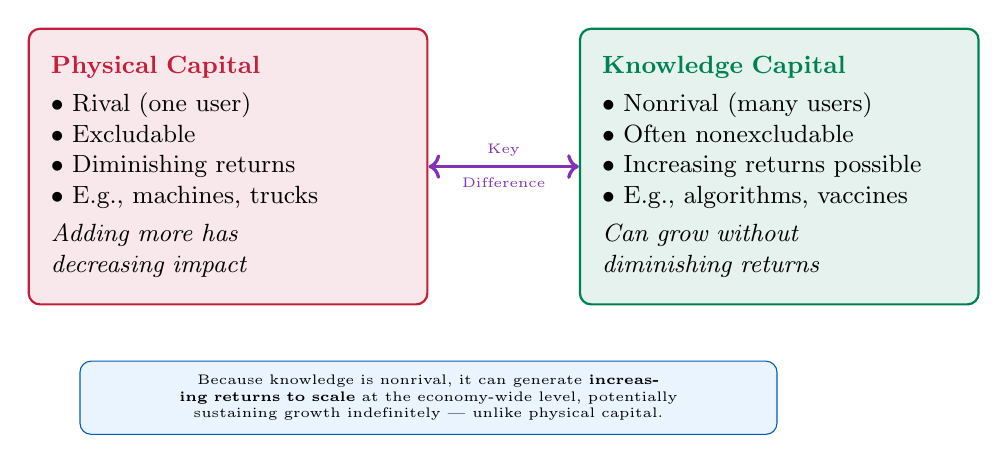
\begin{tikzpicture}[node distance=2cm, every node/.style={font=\small}]
% Physical capital box
\node[draw=canadared, fill=canadared!10, rounded corners, thick,
      text width=4.5cm, minimum height=3.5cm, align=left, inner sep=8pt]
  (phys) at (-3.5,0) {
    \textcolor{canadared}{\textbf{Physical Capital}}\\[3pt]
    $\bullet$ Rival (one user)\\
    $\bullet$ Excludable\\
    $\bullet$ Diminishing returns\\
    $\bullet$ E.g., machines, trucks\\[3pt]
    \textit{Adding more has\\decreasing impact}
  };
% Knowledge capital box
\node[draw=leafgreen, fill=leafgreen!10, rounded corners, thick,
      text width=4.5cm, minimum height=3.5cm, align=left, inner sep=8pt]
  (know) at (3.5,0) {
    \textcolor{leafgreen}{\textbf{Knowledge Capital}}\\[3pt]
    $\bullet$ Nonrival (many users)\\
    $\bullet$ Often nonexcludable\\
    $\bullet$ Increasing returns possible\\
    $\bullet$ E.g., algorithms, vaccines\\[3pt]
    \textit{Can grow without\\diminishing returns}
  };
% Arrow and implication
\draw[<->, shiftpurple, very thick] (phys.east) -- (know.west)
  node[midway, above, font=\tiny, color=shiftpurple] {Key}
  node[midway, below, font=\tiny, color=shiftpurple] {Difference};
\node[below=0.7cm of phys.south east, draw=accent, fill=soft,
      rounded corners, text width=8.5cm, align=center, font=\tiny, inner sep=5pt] {
  Because knowledge is nonrival, it can generate \textbf{increasing returns to scale} at the economy-wide level,
  potentially sustaining growth indefinitely --- unlike physical capital.
};
\end{tikzpicture}
\end{center}
\end{frame}

\begin{frame}{Free-Rider Problem and Underinvestment in R\&D}
\transfade
\begin{itemize}
  \item Because knowledge capital is a \textbf{public good}, firms may not capture its full benefits.
  \item \textbf{Free-rider problem:}
  \begin{itemize}
    \item Firm A invests \$100 million in R\&D to develop a new drug.
    \item Competitors can study the drug, reverse-engineer it, and produce cheaper generics.
    \item Firm A bears the full cost but competitors capture part of the benefit.
  \end{itemize}
  \item \textbf{Result:} Market produces \alert{too little} R\&D relative to the socially optimal amount.
  \item \textbf{Measurement:} Canada's R\&D spending = 1.7\% of GDP (2023) --- below the OECD average of 2.7\% (OECD MSTI, 2024). This gap is a major policy concern.
\end{itemize}
\end{frame}

\begin{frame}{Government's Role: Three Channels}
\transfade
\begin{enumerate}
  \item \textbf{Protecting intellectual property}
  \begin{itemize}
    \item \textbf{Patents:} 20-year exclusive right to produce an invention.
    \begin{itemize}
      \item Encourages innovation by guaranteeing temporary monopoly profits.
      \item E.g., Moderna's mRNA patent gave it time to recoup COVID-19 vaccine R\&D.
    \end{itemize}
    \item \textbf{Copyrights:} protects creative works (books, software, music).
    \item Trade-off: strong IP protection boosts innovation but limits diffusion.
  \end{itemize}
  \item \textbf{Supporting R\&D directly}
  \begin{itemize}
    \item NRC Canada, NSERC grants, SR\&ED tax credit (\$3--4B annually).
  \end{itemize}
  \item \textbf{Subsidizing education}
  \begin{itemize}
    \item Provincial tuition subsidies, federal student loans, immigration of skilled workers.
  \end{itemize}
\end{enumerate}
\end{frame}

% ============================================================
\section{7.4 Why Isn't the Whole World Rich?}
% ============================================================

\begin{frame}{7.4 Learning Objective}
\transfade
\begin{block}{Goal}
Explain economic catch-up and why many poor countries have not experienced rapid growth.
\end{block}
\begin{itemize}
  \item The growth model predicts \textbf{catch-up (convergence)}: poor countries should grow faster.
  \begin{itemize}
    \item Reason: additional capital is more productive at low K/L levels (diminishing returns).
    \item Poor countries can \textbf{import} technologies from rich countries cheaply.
  \end{itemize}
  \item Evidence:
  \begin{itemize}
    \item \alert{Among high-income countries}, convergence has occurred --- South Korea, Taiwan, Ireland.
    \item \alert{For the world as a whole}, convergence has been weak --- many poor countries stagnated.
  \end{itemize}
\end{itemize}
\end{frame}

\begin{frame}{Figure 7.5 -- Convergence Among High-Income Countries}
\begin{center}
\begin{tikzpicture}
\begin{axis}[
  width=0.85\textwidth, height=0.70\textheight,
  xlabel={Real GDP per Capita in 1960 (2017 Int'l \$000s)},
  ylabel={Avg. Annual Growth Rate 1960--2023 (\%)},
  xmin=2, xmax=22, ymin=1, ymax=7,
  grid=both, grid style={dotted,gray!40},
  tick label style={font=\tiny},
  label style={font=\small},
  title style={font=\small\bfseries},
  title={Poor-in-1960 Countries Grew Faster (Conditional Convergence)}
]
% Trend line (negative slope = convergence)
\addplot[goldenrod, dashed, thick, domain=2:22] {-0.18*x + 6.2};
% Country points
\addplot[only marks, mark=*, mark size=2.5pt, accent] coordinates {
  (3.0,6.3)(3.5,5.8)(4.2,5.1)(5.0,4.7)(6.1,4.5)
  (8.0,3.9)(9.5,3.5)(11.0,3.2)(13.0,2.9)(15.0,2.5)
  (17.0,2.2)(20.0,2.0)
};
% Labels
\node[font=\tiny, fill=white] at (axis cs:3.5,6.7) {S. Korea};
\node[font=\tiny, fill=white] at (axis cs:4.5,5.5) {Japan};
\node[font=\tiny, fill=white] at (axis cs:8.5,4.3) {Germany};
\node[font=\tiny, fill=white] at (axis cs:14,3.2) {Canada};
\node[font=\tiny, fill=white] at (axis cs:19,2.4) {USA};
\node[font=\tiny, fill=soft, draw=accent, rounded corners, align=center]
  at (axis cs:11,5.8) {Convergence:\\poorer (in 1960) grew faster};
\end{axis}
\end{tikzpicture}
\end{center}
{\tiny Sources: Maddison Project; IMF WEO. Each point represents one high-income country.}
\end{frame}

\begin{frame}{Why Many Poor Countries Have Not Caught Up}
\transfade
\begin{itemize}
  \item When we extend the analysis to \textbf{all} countries, simple convergence fails:
  \begin{itemize}
    \item Many low-income countries grew very slowly or experienced \textbf{negative} growth.
  \end{itemize}
  \item Economists highlight four key barriers:
\end{itemize}
\begin{columns}
\column{0.48\textwidth}
\begin{block}{\textcolor{canadared}{1. Failure of Rule of Law}}
No property rights, no contract enforcement $\Rightarrow$ entrepreneurs don't invest.
\end{block}
\begin{block}{\textcolor{deeporange}{3. Poor Education \& Health}}
Low human capital $\Rightarrow$ workers can't adopt new technology.
\end{block}
\column{0.48\textwidth}
\begin{block}{\textcolor{shiftpurple}{2. Wars \& Revolutions}}
Destroy capital, disrupt trade, create uncertainty $\Rightarrow$ no investment.
\end{block}
\begin{block}{\textcolor{tealblue}{4. Low Saving \& Investment}}
Vicious cycle: low income $\to$ low saving $\to$ low capital $\to$ low income.
\end{block}
\end{columns}
\end{frame}

\begin{frame}{The Rule of Law: A Prerequisite for Growth}
\transfade
\begin{itemize}
  \item \textbf{Rule of law:} government's ability to enforce laws, especially:
  \begin{itemize}
    \item protecting \textbf{private property rights},
    \item enforcing \textbf{contracts}.
  \end{itemize}
  \item Without strong rule of law:
  \begin{itemize}
    \item entrepreneurs fear expropriation, corruption, and extortion.
    \item They invest \textbf{less} in new businesses and technologies.
  \end{itemize}
  \item \textbf{Evidence:} World Bank Doing Business Index and Property Rights Index show strong positive correlations between rule of law and income levels.
  \item \textbf{Canadian context:} Canada consistently ranks among the top 20 globally for rule of law (World Justice Project, 2024) --- a key reason it attracts foreign investment.
\end{itemize}
\end{frame}

\begin{frame}{Why Have Some High-Income Countries Fallen Behind the U.S.?}
\transfade
\begin{itemize}
  \item Some OECD countries that were close to U.S. productivity in 1990 have \textbf{not} fully caught up:
  \begin{itemize}
    \item Canada's labour productivity (GDP/hour) is approximately \alert{70--75\%} of U.S. levels.
    \item Gap has \textbf{widened} since 2000 (Conference Board of Canada, 2024).
  \end{itemize}
  \item Possible reasons Canada lags:
  \begin{itemize}
    \item Less competition in key sectors (banking, telecom, airlines) --- regulated oligopolies.
    \item Lower business R\&D investment (1.7\% of GDP vs.\ 3.4\% in the U.S.).
    \item Higher marginal tax rates on corporate income.
    \item Less venture capital availability for startups.
    \item Regulatory barriers (interprovincial trade restrictions).
  \end{itemize}
\end{itemize}
\end{frame}

% ============================================================
\section*{Chapter Summary}
% ============================================================

\begin{frame}{Summary}
\transfade
\begin{itemize}
  \item Long-run economic growth is crucial for raising living standards; small differences in growth rates compound into massive income gaps.
  \item Growth models emphasize:
  \begin{itemize}
    \item \textbf{capital deepening} (more K/L, diminishing returns) and
    \item \textbf{technological change} (shifts the production function upward).
  \end{itemize}
  \item \textbf{New growth theory} (Romer) places knowledge capital at the centre: it is nonrival, generating potential increasing returns.
  \item Free-rider problems lead to \alert{underinvestment} in R\&D; governments can help via IP protection, R\&D subsidies, and education.
  \item Convergence holds among high-income countries, but many poor countries are stuck due to:
  \begin{itemize}
    \item weak rule of law, conflict, poor public services, and low saving.
  \end{itemize}
  \item Canada's \alert{labour productivity gap} with the U.S. is a major ongoing policy challenge.
\end{itemize}
\end{frame}

\begin{frame}
\centering
\Huge \textbf{Thank you!}\\[1em]
\large Questions?
\end{frame}

\end{document}
